% Modle pour rapport de Stage de Fin d'Etudes de UTC
% version 0.1
% 2012-07-12
% par ZHU Yinan (zhuyinan1988@gmail.com)

\documentclass[12pt,oneside,a4paper]{book}
%Chargement des packages
\usepackage[utf8]{inputenc} % l'encodage des fichiers est utf-8, mettre [latin1] si necessaire
\usepackage[french]{babel} %le rapport est en français 
\usepackage{amsmath}
\usepackage{amsfonts}
\usepackage{amssymb}
\usepackage{graphicx} %pour afficher des images
\usepackage{float}	%pour forcer le placement des images.
\usepackage{geometry} %pour la modification des marges
\usepackage{fancyhdr} %pour modification des pieds de page
\usepackage{longtable}
\usepackage{listings}
\usepackage{subfigure}
%\usepackage[Sonny]{fncychap}
\usepackage{hyperref} %pour que les références soient des liens hypertextes
\usepackage[usenames,dvipsnames]{color} % pour les textes en gris
\hypersetup{backref, pdfborder=0 0 0}
\usepackage{ragged2e}



% Comment utiliser : 
% - la page de titre est à personnaliser (title/title.tex)
% - le contenu est à rédiger dans le répertoire pages/, s'inspirer des exemples présents dans ce modèle.
% - les annexes sont à rédiger dans le répertoire appendix/
% - la bibliographie utilise BibTex (fichier biblio.bib)
% - les variables suivantes sont à remplir :
\newcommand{\TitreRapport}{Rapport de stage TN10}
\newcommand{\DateRapport}{2012}
\newcommand{\AuteurRapport}{Yinan ZHU}
\newcommand{\NomEntreprise}{Data Gest}

%définition des marges
\geometry{hmargin=2.5cm, vmargin=2.5cm } 

%utilisation des puces anglaises.
%attention, il faut avoir une version récente de frenchb.ldf. 
\frenchbsetup{StandardItemLabels}

%Définition des en-têtes et pieds de page
\renewcommand{\headrulewidth}{0.5pt}
\renewcommand{\footrulewidth}{0.5pt}
%\fancyhead[C]{ \textcolor{Gray}{\small\TitreRapport}}
\fancyfoot[LE, RO]{ \textcolor{Gray}{ \small\AuteurRapport ~~ \vline ~~ UTC ~~ \vline ~~ \DateRapport }}

\fancyfoot[C]{\thepage}
\fancyfoot[RE, LO]{
\includegraphics[width=1.8cm]{style/images/logo_utc.png}}
%\fancyhead[LE,RO]{\thepage}
\fancyhead[LO]{\rightmark}
\fancyhead[RE]{\leftmark}


%\fancyhead[L,R]{}


% définition du tire, de la date et de l'auteur du document
\title{\TitreRapport}
\date{\DateRapport}
\author{\AuteurRapport}

\makeatletter
\newcommand{\HRule}{\rule{\linewidth}{2.5mm}}
\renewcommand\maketitle{
  \begin{titlepage}
    \begin{center}
      
\includegraphics[width=7.2cm]{title/images/logo_utc.png}
      \hspace{\stretch{1}}
      %
\includegraphics[width=5.2cm]{title/images/data-gest.jpg}

      \vspace{\stretch{0.5}}

      \begin{tabular*}{1.0\textwidth}{l @{\extracolsep{\fill}} r}
        Université de téchnologie de Compiègne \\ 			%	& \NomEntreprise 				\\
        UTC \@date 							%& La Plaine de Saint Dennis 		\\
      \end{tabular*}

      \vspace{\stretch{1.5}}
      % Title
      \begin{flushright}
        {\huge \bfseries \@title\\}
        \HRule \\[0.5cm]
        {\Large \it Rapport Final de Stage de Fin d'études \\[3.5cm]}
      \end{flushright}
      %{\large \it \@author\\}
      \begin{minipage}{1\textwidth}
        \begin{flushright} \large

          \@author \\
          Système Réseaux Informatique  \\[7.5cm]
        \end{flushright}
        \begin{flushleft}
          \emph{Tutrise:} Mme.~Angélique \textsc{Ruton} \\
          \emph{Suiveur UTC:} M.~Boris \textsc{Vidolov} \\
          \emph{Entreprise:} DATA-GEST  \\

        \end{flushleft}
      \end{minipage}
      \vspace{\stretch{2}}
      %
\includegraphics[width=1.0\textwidth]{title/images/logo_illustration.png}
      \vspace{\stretch{2}}


    \end{center}\par

  \end{titlepage}
  \setcounter{footnote}{0}

%  \global\let\thanks\relax
%  \global\let\maketitle\relax
%  \global\let\@thanks\@empty
%  \global\let\@author\@empty
%  \global\let\@date\@empty
%  \global\let\@title\@empty
%  \global\let\title\relax
%  \global\let\author\relax
%  \global\let\date\relax
%  \global\let\and\relax
}


\makeatother


\begin{document}

\pagestyle{fancy}
\maketitle
\frontmatter
\chapter{Remerciements}
%\renewcommand{\baselinestretch}{3.5}
\setlength{\parskip}{0.5\baselineskip}

%Tout d'abord, je dois remercier à ma tutrice, Angélique RUTON, elle m'a donné beaucoup d'avis dans la domaine de programmation, et aussi dans la partie de conception. En plus, j'ai approfondi aussi dans la gestion de projet. Non seulement elle m'a donné suggestions dans la partie technique, mais aussi dans m'a donné les suggestions pour mon  carrier futur duquel j'ai tiré de grands profits.  

%Ensuite, je dois remercier à mon collègue, Edouard KOMBO, qui est très chaleureux et humoristique. Il m'a  aidé souvent si j'ai eu les problème dans la programmation. En plus, il m'a donné un coup de main afin que je peux pré-embauche chez DATA-GEST


\paragraph{}
Mes remerciements s’adressent en premier lieu à ma tutrice de stage,  Madame Angélique RUTON, chef de projet de pôle web de la société DATA-GEST, pour sa confiance et ses conseils qui m’ont permis de progresser sans cesse durant ces 6 mois de stage.

\paragraph{} 
Je remercie également Monsieur Boris VIDOLOV pour l’aide et les conseils concernant les missions évoquées, le dans ce rapport, qu’il m’a apporté lors des différents suivis.

\paragraph{} 
J’exprime également ma gratitude à l’égard de l’ensemble de l'équipe pôle web et aussi service commercial pour leur précieuse aide ainsi que leur sympathie qui ont favorisées mon intégration dans l’entreprise.

\chapter{Résumé du rapport :}
%Insérez ici le résumé en français
\flushleft
Le rapport finale  contient tous les parties pendant mon stage fin d'étude.\\
Il est consisté en n chapitres :
\begin{description}
  \item[Chapitre 1] Un bref introduction de l'entreprise et aussi le sujet de stage
  \item[Chapitre 2] Un bref introduction de l'entreprise et aussi le sujet de stage
  \item[Chapitre 4] Un bref introduction de l'entreprise et aussi le sujet de stage
  \item[Chapitre 3] Un bref introduction de l'entreprise et aussi le sujet de stage
\end{description}
\subsubsection*{Mots-clés libres :}
%Insérez ici les mots clés en français (séparés par des points-virgules)
Gestion du projet; PHP; HTML; SVN; CSS; AJAX; KDOMOTIV

\tableofcontents
\listoffigures
\listoftables
\mainmatter
\chapter{Introduction}\thispagestyle{fancy}

\section{Introduction d'entreprise}
\justifying

Spécialisée dans le marketing opérationnel, DATA-GEST évolue depuis plusieurs années sur le marché de la stimulation des ventes et du cadeau d’affaires.\\[2ex]

\subsection{Mission principale}
\paragraph{}
\begin{description}
  \item[Fidélisation clientèle]Les programmes de fidélisation subissent depuis quelques années une véritable restructuration.

Au delà du simple aspect transactionnel on s’ouvre de plus en plus au relationnel.

Data-Gest vous accompagne dans votre démarche, de la réflexion en amont à la mise en place opérationnelle.

  \item[Motivation commerciale]La stimulation des ventes est un excellent outil d'incitation à la performance. La mécanique doit être simple, sans artifices et appréhendable par tous.

Avec un objectif d'efficacité et de rentabilité, Data-Gest met à votre disposition différents outils packagés ou complètement personnalisés à votre projet.
  \item[Parrainages clients]Ce concept qui consiste à transformer chaque client fidèle en prescripteur, capable d'apporter des prospects clés en main, est un outil de conquête redoutable.

Data-Gest vous accompagne dans la mise en place et le suivi de vos campagnes de parrainages.
  \item[Animation réseaux]Animer ses circuits de distribution pour créer une adhésion forte entre la marque et son réseau et sceller ainsi une collaboration qui profite aux deux parties.

Data-Gest vous accompagne dans votre stratégie en vous proposant les méthodes et les outils d'animation et de stimulation les plus adaptés.
  \item[Cadeaux d'affaire]
Le cadeau d'affaires est un don à caractère événementiel, réalisé dans le but de remercier une clientèle de sa fidélité à l'entreprise. Notre département cadeaux d'affaires offre toute une gamme d'articles issus d'univers variés : high-tech, décoration, gastronomie, articles de bureau, maroquinerie, développement durable …
Selon votre problématique, nos équipes vous proposeront le choix entre plusieurs formules packagées ou sur mesure. 

\end{description}
\subsubsection{Titre de niveau 3}
Isdem diebus Apollinaris Domitiani gener, paulo ante agens palatii Caesaris curam, ad Mesopotamiam missus a socero per militares numeros immodice scrutabatur, an quaedam altiora meditantis iam Galli secreta susceperint scripta, qui conpertis Antiochiae gestis per minorem Armeniam lapsus Constantinopolim petit exindeque per protectores retractus artissime tenebatur.

\begin{itemize}
\item Liste a puces 1
			\begin{itemize}
			\item Liste a puces 2
						\begin{itemize}
						\item Liste a puces 3
						\end{itemize}
			\end{itemize}
\end{itemize} 

\paragraph{Titre de niveau 4}
Non ergo erunt homines deliciis diffluentes audiendi, si quando de amicitia, quam nec usu nec ratione habent cognitam, disputabunt.

\begin{figure}[H]
	\center
	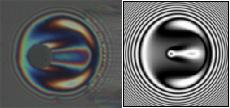
\includegraphics[width=5cm]{body/images/figure_example.png} 
	\caption{Exemple de figure avec légende}
	\label{fig:exemple}
\end{figure}

\subparagraph{Titre de niveau 5}

Isdem diebus Apollinaris Domitiani gener, paulo ante agens palatii Caesaris curam, ad Mesopotamiam missus a socero per militares numeros immodice scrutabatur, an quaedam altiora meditantis iam Galli secreta susceperint scripta, qui conpertis Antiochiae gestis per minorem Armeniam lapsus Constantinopolim petit exindeque per protectores retractus artissime tenebatur.

Titre de niveau 6
Non ergo erunt homines deliciis diffluentes audiendi,

\subsection{Savoir-faire de Data-Gest}
\paragraph{}
Data Gest se caractérise par son approche concrète et globale du marketing opérationnel.
Ses différents pôles de compétences transversales sont entièrement internalisés :\\[1em]
\begin{itemize}
  \item Pôle stratégique pour vous accompagner dans la définition, la réalisation et la mise en place de vos actions marketing.
  \item Studio création graphique et conception web : pour dynamiser vos supports de communication.
  \item Division opérationnelle pour le suivi commercial et logistique de vos campagnes.
  \item Département dotations / cadeaux d’affaires : base de données cadeaux de plusieurs milliers d'articles issus d'univers variés (maroquinerie, bricolage, high-tech, électroménager, horlogerie....).

\end{itemize}




\section{Introduction du sujet}
\justifying
\subsection{Description}
\paragraph{}
Data-Gest est une agence spécialisée dans le marketing opérationnel (programmes de fidélisation et de parrainages, challenges commerciaux'). Depuis sa création en 2000, la société est en forte croissance et travaille essentiellement avec de grand comptes ( Allianz, La Poste, Air France')
\paragraph{}


Au sein du « département Web \& nouvelles technologies » et en liaison avec le pôle Marketing et Commercial, je suis en charge du développement et de l'évolution de nos solutions Web. 
Mes missions principales :
\begin{figure}
  \centering
  \subfigure[Air france]{\label{fig:air france}
\includegraphics[width=0.3\textwidth]{body/images/air-france-logo.jpg}}                
  \subfigure[Allianz]{\label{fig:Allianz}
\includegraphics[width=0.3\textwidth]{body/images/allianz.jpeg}}
  \subfigure[La poste]{\label{fig:mouse}
\includegraphics[width=0.3\textwidth]{body/images/laposte.png}}
  \caption{Partenaire de Data-Gest}
  \label{fig:Partenaire de Data-Gest}
\end{figure}

\begin{itemize}
  \item [-]Prise de brief 
  \item [-]Rédaction des spécifications fonctionnelles et des story-boards, 
  \item [-]Contrôle qualité et test, 
  \item [-]Intégration XHTML / CSS
  \item [-]bon respect de la méthodologie projet,
  \item [-]respect des budgets et des délais, 
\end{itemize}

\subsection{Objet final}
\paragraph{}
Bien amélioration du frame-work de l'entreprise : KdoMotive
Réaliser le projet pendant le période de stage. Et corriger le bug, tester le site, et aussi améliorer les codes

\subsection{Organisation du travail}
Déroulement:

TODO: diagramme du gantt
ou table de bilan
%\input{body/pages/chapitre-intro/intro-sujet/}



\chapter{Pré études}\thispagestyle{fancy}
\paragraph{}
Avant de commencer le travail, j'ai pris 3 semaine afin de bien comprendre comment fonctionne les mécanismes de pôle web chez Data-Gest.Ci-dessous sont les parties principales.

\section{Serveur}
%\justifying

%Spécialisée dans le marketing opérationnel, DATA-GEST évolue depuis plusieurs années sur le marché de la stimulation des ventes et du cadeau d’affaires.\\[2ex]

\subsection{Serveur local}


\subsubsection{Infrastructure}
Il y a trois serveurs locals chez Data-Gest. 
\begin{description}
\item[•]DATAGESTSRV01
\item[•]DATAGESTSRV02
\item[•]SRV-NAVISION
\end{description}


\subparagraph{}
L'infrastructure est déjà configurée en mode failover. C'est à dire que l'ip sur lequel le service est hébergé est routé sur le
serveur princial (ns26393.ovh.net). En cas de panne du serveur principale l'adresse ip est routée vers le serveur
secondaire. Par conséquent il faudra configurer les domaines de production pour qu'ils dirigent vers l'adresse IP
178.33.251.180.




%\begin{itemize}
%\item Liste a puces 1
%			\begin{itemize}
%			\item Liste a puces 2
%						\begin{itemize}
%						\item Liste a puces 3
%						\end{itemize}
%			\end{itemize}
%\end{itemize} 
%
%\paragraph{Titre de niveau 4}
%Non ergo erunt homines deliciis diffluentes audiendi, si quando de amicitia, quam nec usu nec ratione habent cognitam, disputabunt.
%
%\begin{figure}[H]
%	\center
%	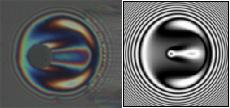
\includegraphics[width=5cm]{body/images/figure_example.png} 
%	\caption{Exemple de figure avec légende}
%	\label{fig:exemple}
%\end{figure}
%
%\subparagraph{Titre de niveau 5}
%
%Isdem diebus Apollinaris Domitiani gener, paulo ante agens palatii Caesaris curam, ad Mesopotamiam missus a socero per militares numeros immodice scrutabatur, an quaedam altiora meditantis iam Galli secreta susceperint scripta, qui conpertis Antiochiae gestis per minorem Armeniam lapsus Constantinopolim petit exindeque per protectores retractus artissime tenebatur.
%
%Titre de niveau 6
%Non ergo erunt homines deliciis diffluentes audiendi,




\subsection{Serveur distant}
\paragraph{}
Les serveurs de distants de Data-Gest sont gérés par OVH. Les services suivant sont déjà mis en place par défaut: 

%\begin{itemize}
%\item Liste a puces 1
%			\begin{itemize}
%			\item Liste a puces 2
%						\begin{itemize}
%						\item Liste a puces 3
%						\end{itemize}
%			\end{itemize}
%\end{itemize} 
%
%\paragraph{Titre de niveau 4}
%Non ergo erunt homines deliciis diffluentes audiendi, si quando de amicitia, quam nec usu nec ratione habent cognitam, disputabunt.
%
%\begin{figure}[H]
%	\center
%	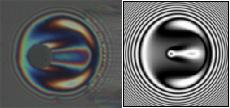
\includegraphics[width=5cm]{body/images/figure_example.png} 
%	\caption{Exemple de figure avec légende}
%	\label{fig:exemple}
%\end{figure}
%
%\subparagraph{Titre de niveau 5}
%
%Isdem diebus Apollinaris Domitiani gener, paulo ante agens palatii Caesaris curam, ad Mesopotamiam missus a socero per militares numeros immodice scrutabatur, an quaedam altiora meditantis iam Galli secreta susceperint scripta, qui conpertis Antiochiae gestis per minorem Armeniam lapsus Constantinopolim petit exindeque per protectores retractus artissime tenebatur.
%
%Titre de niveau 6
%Non ergo erunt homines deliciis diffluentes audiendi,

\subsection{Savoir-faire de Data-Gest}
\paragraph{}
Data Gest se caractérise par son approche concrète et globale du marketing opérationnel.
Ses différents pôles de compétences transversales sont entièrement internalisés :\\[1em]
\begin{itemize}
  \item Pôle stratégique pour vous accompagner dans la définition, la réalisation et la mise en place de vos actions marketing.
  \item Studio création graphique et conception web : pour dynamiser vos supports de communication.
  \item Division opérationnelle pour le suivi commercial et logistique de vos campagnes.
  \item Département dotations / cadeaux d’affaires : base de données cadeaux de plusieurs milliers d'articles issus d'univers variés (maroquinerie, bricolage, high-tech, électroménager, horlogerie....).

\end{itemize}



\section{ModuleDG}
%\justifying

\paragraph{}
ModuleDG est un web service développé par Data-Gest qui sert à :
\begin{itemize}
\item [-] Gestion des commandes envoyé depuis chaque site.
\item [-] Gestion de la base de donnée de cadeaux total. 
\item [-] Gestion de la sélection de cadeaux de chaque site.
\end{itemize}

\paragraph{}
La fonctionnalité est bien illustré dans le figure suivant.

[TODO: structure de ModuleDG et chaque site]

En fait chaque site a une sélection de cadeaux qui est géré par  ModuleDG. Quand le client de chaque site valide un commande, il sera passé à moduleDG pour le contrôler. 



\chapter{Déroulement}\thispagestyle{fancy}

\paragraph{}
Cette chapitre explique les travaux principale pendant mon stage. Il se compose de trois sections. Tous d'abord, j'ai installé et configuré un environnement de développement afin de améliorer l'efficacité. Ensuit, le travaille principale est l'amélioration du framework KdoMotiv Médium. Dernièrement, c'est quelque projets lesquels j'ai réalisé par KdoMotiv.

\section[Configuration]{Configuration de l'environnement}

\subsection{Installer un serveur linux local}
\paragraph{}
Comme le problème j'ai expliqué dans le chapitre avant, ce n'est pas très pratique avec un serveur disant sans droits ou un serveur local avec système exploitation de windows.
Auparavant, quand les collègue de pôle web avait le problème sur quelque site, ils doivent communiquer directement chez notre pôle. En plus, il n'y a rien de trace ou histoire sur le problème. 
Par conséquent, j'ai choisi un ordinateur qui n'est utilisé plus comme un nouveau serveur local. 

Lorsque ubuntu est un système d'exploitation intuitif et sécurisé, idéal pour les ordinateurs de bureau, les serveurs, les netbooks et les ordinateurs portables. En plus, Ubuntu est libre, gratuit, et est composé de logiciels qui le sont également.

J'ai décidé d'installer ubuntu serveur 10.04(LTS\footnote{Long Term Support}) sur serveur local.

\subsubsection{Partition}
En fait, comme le serveur local n'est pas très puissant,il a juste 2G de RAM de ce PC.  il faut l'attribuer 2G de swap. La partition de disque est comme la table suivant.

\begin{table}[htbp]
\centering
\begin{tabular}{ll}
  \toprule
  Partition & G\\
  \midrule
	/ & 30 \\ 
	\hline 
	swap & 2 \\ 
	\hline 
	/var & 10 \\ 
	\hline 
	/tmp & 5 \\ 
	\hline 
	/home & reste \\
  \bottomrule
\end{tabular}
 \caption{\label{tab:Partition du serveur}Partition du serveur}
\end{table}

\subsubsection{Installation de l'environnement LAMP + PhpMyAdmin}
LAMP est un acronyme désignant un ensemble de logiciels libres permettant de construire des serveurs de sites web. L'acronyme original se réfère aux logiciels suivants :
\begin{itemize}
\item[•] Linux 
\item[•] Apache 
\item[•] MySQL 
\item[•] PHP 
\end{itemize}
Sur ce serveur local, on a aussi besoin de debuger le site php ou développer quelque fonctions de php sert à traiter les données locales. Il faut configurer un environnement plus proche ou similaire que l'environnement LAMP sur serveur distant. Pourquoi mettre un environnement plus similaire que celui sur serveur production? Au cas où si on va déployer ce que on a développer sur serveur local, mais ne fonctionne pas sur serveur de production. 

D'ailleurs, afin de contrôler le serveur plus facilement, j'ai aussi installé le OPENSSH. Après cette étap, je peux faire tous les opérations sur ma poste avec PuTTY\footnote{PuTTY est un émulateur de terminal doublé d'un client pour les protocoles SSH, Telnet, rlogin, et TCP brut.}

Mais, il y a encore de un peu de problème de ce serveur. Tous d'abord, comme c'est un PC dans réseau local, on n'a pas fixer l'adresse IP de cette machine. S'il a éprouvé la situation de coupure d'électricité de week-end, et le serveur a redémarré automatiquement, l'adresse IP de cette machine serait changé à cause de DHCP. C'est-à-dire chaque fois, on doit informer à les autre département du changement de l'adresse IP de serveur local.

Ce n'est pas pratique. La solution sera fixé l'adresse ip depuis la configuration du routeur.



\subsubsection{Installation de Ruby on Rails et RedMine}
Comme le problème lequel j'ai déjà expliqué dans le chapitre avant, ce n'est pas pratique de communiquer entre différent pôle  et suivre ou tracer des bugs de tous les projets. 

Par conséquent, j'ai trouver deux applications web candidats qui sert à la gestion de projet. Une est RedMine qui est programmé par Ruby, l'autre est Trac qui est programmé par python. Finalement, j'ai fixé d'utiliser RedMine dû à son plus agréable interface.  

Vu que RedMine est une web application sous framework Ruby on Rails. Il faut configurer la framework de ROR sur serveur local. 

Après l'installation et la configuration du ROR, la mise en place de Redmine est simple. Suivi les instructions depuis le site officiel de Redmine, c'est simple de mettre en œuvre. 

Ensuite, j'ai déposé tous les projets actuels de Data-Gest afin de gérer et tracer sur RedMine. On peut aussi apercevoir les anomalies, les évolution, les assistances de chaque projet.
\begin{figure}[hbtp]
\center
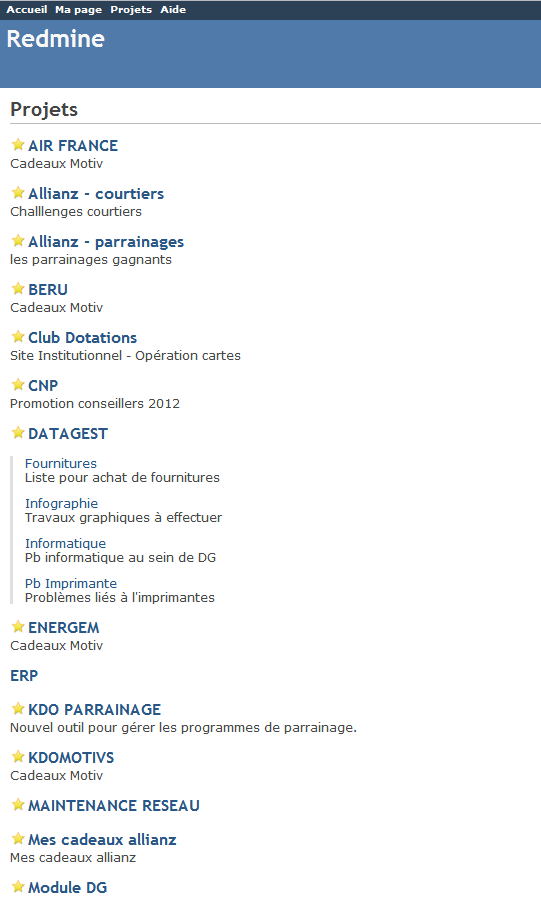
\includegraphics[width=10cm]{body/images/redmine-accueil.PNG}
\caption{Acceuil de Redmine}
\end{figure}



Cependant, quand j'ai essayé d'ajouter un ticket sur redmine à la fin du test, je n'ai reçu aucune  mail de notification lorsque le changement de ticket.

\subsubsection{Installation du serveur mail(Postfix) local}
Afin de fixer le problème que j'avais avant concernent le mails. J'ai installé le Postfix comme le serveur de messagerie électronique au remplacement du serveur \textbf{Sendmail}, vu qu'il est plus léger et plus stable. La configuration de Postfix en détail est dans annexe.

\subsubsection{Résume}
Étant donné que le serveur local peut juste être visité pas adresse IP, mais il y a plusieurs services sur ce serveur. Par conséquence, j'ai configuré les différent portes de Apache ou on peut y accéder pour utiliser le différent service. Par exemple, si on va accéder à PhpMyAdmin\footnote{Interface graphique pour gérer MySQL}, on peut juste ajout la porte correspondant après l'adresse IP.

\begin{table}[htbp]
\centering
\begin{tabular}{ll}
  \toprule
  Porte & Service\\
  \midrule
	80(Par défaut) & l'application RedMine \\ 	 
	8080 & CMS Drupal, développement de site par Drupal \\ 	 
	8888 & PhpMyAdmin, interface graphique pour la gestion Base de donnée \\ 	 
  \bottomrule
\end{tabular}
 \caption{\label{tab:Service de différents portes}Service de différents portes}
\end{table}

\subsection{Configuration un serveur SVN sur seveur distant}
\paragraph{}
Quand le serveur distant OHV est mise en œuvre, le SVN est déjà pré-installé sur le serveur dev, c'est-à-dire on peut contrôler lès version de projets que on a déjà développé. Mais on a pas bien communiqué avec l'administrateur réseaux d'OVH, et on n'a utilisé jamais depuis un an. Après le nouveaux chef de gestion de projet est arrivé, on l'a décidé de reprendre. 

Mais il semble que le SVN sur serveur dev distant est mal configuré, il y a juste un dépôt de subvention par défaut sur le serveur. En plus, on a pas de droit de le configuré soi-même. Par conséquence, on a demandé  à l'administrateur réseaux d'ovh de nous donner tous les droits d'en contrôler. 

\subsubsection{Fichier de conf}
Après on a gagné les droit de configuration dans le répertoire de SVN, on a créé un dépôt qui sert à notre premier projet lequel on voudrait contrôler la version en ligne de commande. Dans le répertoire "\textbf{conf}" de ce dépôt subvention, on peut ajouter les utilisateurs qui peuvent faire les action "commit" à ce dépôt  ou "check out" depuis ce dépôt. 
\begin{figure}[hbtp]
\center
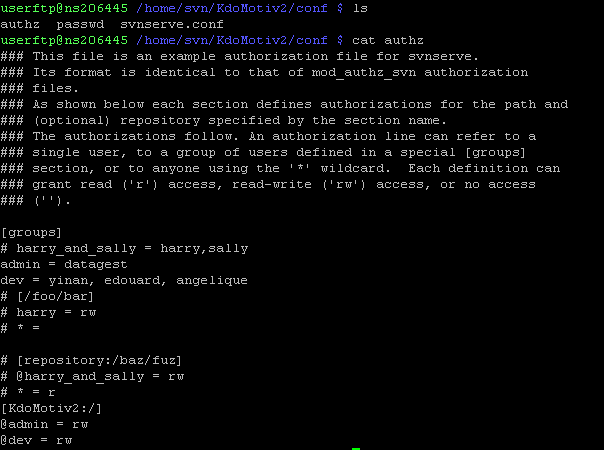
\includegraphics[width=10cm]{body/images/conf-svn.png}
\caption{fichier conf SVN}
\end{figure}


\subsubsection{Problème de permission de répertoire }
On a installé TortoiseSVN comme le logiciel de côté client.  Mais on a eu le problème de la permission de commit pendant le commit. En fait, le dépôt on a créé est dans le groupe de "user". Mais quand on fait un commit depuis côté client, c'est le utilisateur svn dans groupe svn qui le fait par défaut, il n'a pas de droit d'écrire et lire dans répertoire de dépôt.

On doit lancé a commande dans linux afin de changer l'utilisateur et le groupe d'une répertoire dans le dépôt. 

\begin{figure}[hbtp]
\center
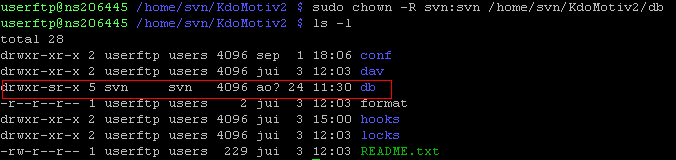
\includegraphics[width=10cm]{body/images/svn-problem-permission.png}
\caption{Changer groupe de répertoire}
\end{figure}

\subsubsection{WEBSVN}
WEBSVN est un interface graphique permettant de visualiser les versions des projets. Il est pointé vers le répertoire de dépôt de SVN.
\begin{figure}[hbtp]
\center
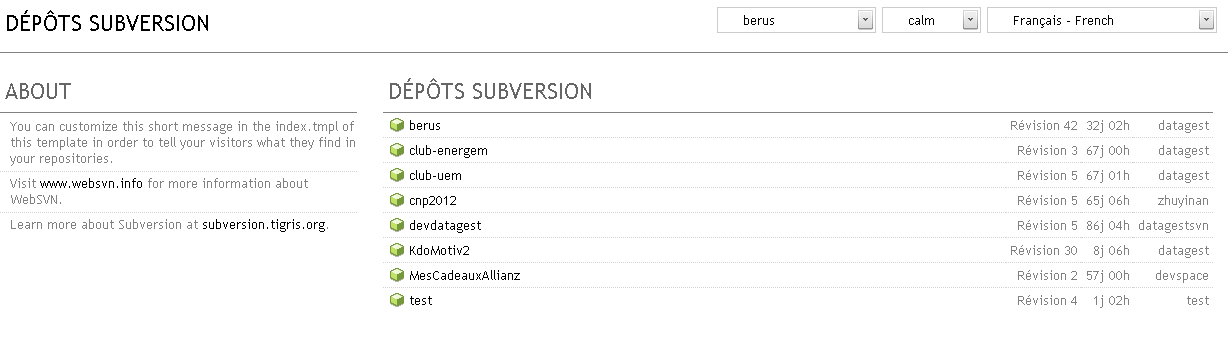
\includegraphics[width=15cm]{body/images/websvn.png}
\caption{Interface WEBSVN}
\end{figure}


\subsubsection{HOOK}
Un hook (littéralement crochet) permet de lancer un programme personnalisé au moment précis où le programme principal à la tâche de l’exécuter. Dans le cas de svn les hooks sont applicables sur les évènements de contrôle de version( commit , changement de révision, lock). On peut le comparer à la notion de trigger en sql.
On utilise "hook" chaque fois que on fait un commit de local à serveur distant afin de aussi mettre à jour de modification dans le répertoire où le site est situé. C'est très pratique pour le debug.

Ce que on a utilisé dans hook est l'événement \textbf{post-commit} , une notification du succés de la transaction de commit. Généralement utilisé pour envoyer un mail à un administrateur ou synchroniser le site 


\subsection{Création de la documentation du Data-Gest}
\paragraph{}
Avant je suis arrivé, il n'y a rien de documentation de pôle web chez Data-Gest, c'est la raison que je voudrais créer la documentation de noter ce que j'ai fait. Dans variés types des applications de wiki, j'ai choisi dokuwiki comme le wiki de Data-Gest basé sur les raison suivant.
\begin{itemize}
\item [-] C'est un moteur de wiki libre sous licence GUN GPL
\item [-] Simple à utiliser et déployer comme il est développé en PHP.
\item [-] Le plus important avantages est que toutes les données sont stockées dans des fichiers texte, et donc aucune base de données n’est nécessaire. C'est très pratique pour la migration.
\end{itemize}

\paragraph{}
Ce que j'ai rédigé principal dans le wiki sont la gestion de SVN sur serveur distant, les informations de serveur local et serveur distant, et aussi certain informations très important que on doit le noter. 

\begin{figure}[hbtp]
\center

\includegraphics[scale=1]{body/images/dukowiki.png}
\caption{Dokuwiki}
\end{figure}

\newpage

\section[Amélioration KdoMotiv]{Amélioration du framework KdoMotiv}
La mission principale pendant mon stage est d'améliorer le framework KdoMotiv médium. 


\newpage
\section{Projets}


\backmatter
\chapter{Conclusion}
%\addcontentsline{toc}{section}{Conclusion}

Lorsque de mon stage de fin d'étude de 6 mois, j'ai appris beaucoup de chose.

Tout d'abord, j'arrive de intégration dans une équipe rapidement. Auparavant, à cause de problème de mon niveau de langue, ça prend du temps de bien comprendre le sujet et la fonctionnalité du groupe. Par conséquence, ce n'est pas pratique de intégrer dans un groupe de développement. 

Grâce à l'augmentation de niveau de mon langue français  et aussi beaucoup de méthodologie j'ai appris pendant ma formation dans filière SRI à UTC, j'arrive de intégrer dans le développement rapidement après un mois de pré études chez Data-Gest, et aussi à l'aide de mon tuteur qui m'a expliqué la  fonctionnalité et structure de framework en détail avec patience. 

Deuxièmement, j'arrive de  mettre en pratique mes connaissances théoriques acquises durant mes études à UTC . Surtout dans la partie de l'administration de système et configuration du réseaux. Après 6 mois de m'entraîner, je peux bien maîtriser VIM, et aussi beaucoup de méthodes techniques d'utiliser BASH commandes sous Linux.

Troisième, mon niveau de programmation est augmenté. Surtout dans la programmation orienté objet. Au début, j'avais juste un concept de POO, après avoir pratiqué 6 mois pendant mon stage, ma connaissance de POO est enrichi.

Dernièrement, j'ai bien pratiqué la méthodologie de la gestion du projet. Pendant mon stage, il faut souvent travailler sur plusieurs sujet simultanément. En utilisant la méthodologie, j'arrive de coordonner des différents projets. 

Le stage fin d'étude est un excellent souvenir, il constitue désormais une expérience professionnelle valorisante et encourageante pour mon carrière future. J'ai vécu une expérience enrichissante de travail pour la suite et mes futurs emplois. 

En résumé, je trouve que ce stage a été très bénéfique. Et aussi, je tiens à exprimer ma satisfaction d'avoir pu travaillé dans de bonnes conditions matérielles et un environnement agréable



\bibliographystyle{plain}
\bibliography{biblio}\addcontentsline{toc}{chapter}{Bibliographie} 
\appendix
\chapter{Annexe}

\section{Configuration du Postfix}

\lstinputlisting[language=bash, frame=shadowbox, numbers=left, numberstyle=\tiny, stringstyle=\color{red}]{appendix/main.cf}


\end{document}
